\documentclass{article}

\usepackage[english]{babel}
\usepackage{hyperref}
\usepackage{graphicx}
%\usepackage{accsupp}
\usepackage{fancyhdr}
\pagestyle{fancy}
%\usepackage{xcolor}
%\usepackage{xparse}
%\usepackage{tabularx}
\usepackage{longtable}
\fancyhf{}


\chead{
\includegraphics[width=1cm]{images/icon-black.pdf}}
\cfoot{\thepage}

\author{phseiff\\ \href{https://phseiff.com}{from phseiff.com}}

\title{\begin{center}
           %\BeginAccSupp{method=plain,Alt={\{gender*render\}\\Specification}}
           
\includegraphics{images/title-black.pdf}
           %\EndAccSupp{}
\end{center} Template system and implementation specification for rendering gender-neutral email templates with pronoun information}

\begin{document}
\maketitle
\tableofcontents

\section{Abstract}

    Our society, as well as the way we perceive gender, are steadily evolving.
    This evolution does not hold in light of technological questions, and it is our -the "IT people"'s duty- to address and do our best to solve the social issues that arise from our technology.
    One such technology are email- and other text templates, which are becoming increasingly popular to automate customer interactions of any kind, be it in newsletters, notifications or program menus.
    Many such templates are gender-specific, in that they address the reader in a gendered fashion ("Dear Mrs. Dursley, ...").
    Such templates are relatively easily implemented by providing two versions of the email, one for every binary gender.
    However, some texts are far more complicated, because they address multiple people (each with their own unknown at the time of writing), or people in the third person (throwing their pronouns into the mix).
    In addition, an increasingly height amount of people use non-binary pronouns, or gender-neutral pronouns, many of whom might now yet be discovered at the time of writing, which makes these people marginalized when it comes to being correctly addressed even in automated emails.\\

    This creates the requirement for creating template systems for the english language, and, in extention, any language (since all languages work differently), that support writing complex texts in a gender-neutral fashion and later "render" them to correctly gendered texts.\\

    \{gender*render\} is an attempt at creating one such template language, including a Specification, to serve as a proof of concept as well as a starting point for people who want to implement similar things.
    The vision behind this proof of concept is not only to show \emph{how} addressing people with unconventional preferred pronouns can be automized, but also to show \emph{that} it can be easily automized, to debunk the myth that properly addressing non-binary people in an automated fashion is simply technically impossible.

\section{Requirements}

    There are multiple requirements for such a template language, whom I will list here, including short explanation of why they are required wherever I deem it necessary:

    \begin{itemize}
        \item The language must be easy to use even for less tech affine people.
              This means that the atoms of the language, such as tags et cetera, must be as short as possible, and should not clash with commonly used words or signs, so the amount of escape characters the user needs to use is minimal.
        \item The language must support different scenarios:
        \begin{itemize}
            \item One person being addressed versus multiple people being addressed
            \item Only people mentioned in first person, only people mentioned in third person, or a mixture of both
            \item Everyone using pronouns versus some people preferring not to use any pronouns
        \end{itemize}
        \item The fact that multiple scenarios are supported may not make using the template language for only a subset of them more complicated that it needs to be.
        \item Rendering templates may only require the information needed for rendering the template.
        For example, rendering a template that never addresses anyone in the first person should not require providing information as to whether the person goes by "Mr", "Mrs" or any other form of address.
        This is especially relevant since users do not want and should not need to require more information that necessary for rendering the templates, especially considering the intimate nature of preferred pronouns.
        \item The syntax should be describable using a context-free grammar in conjunctive normal form, which allows easy syntax checking and syntax highlighting.
        \item The data containing a persons preferred pronouns should be given in a widely-used, standardized format, such as JSON.
    \end{itemize}

\section{Design Decisions}

    The following decisions where made based on the the technical requirements ruled out in the corresponding section:

    \begin{itemize}
        \item The language uses a syntax similar to pythons build-in string formatting syntax, using curly brackets to annotate gender-specific parts of a sentence.
        Backslashes are used as escape characters for the rare occurrences where curly brackets are actually needed.
        \item In addition to terms like "possessive pronoun", using the gender-neutral form ("their") in tags is supported, potentially making texts more fluid to write and easier to read in their un-rendered form.
        \item If tags contain IDs to annotate which person is referred to, a mapping of IDs to pronoun preferences is accepted for rendering.
        If no such IDs are added to the document because only one person of unknown gender is addressed in the document, the pronoun preferences are directly accepted by the renderer, without having to be part of a person-to-pronoun-mapping.
        This supports referring to multiple persons in one text without making the writing of texts that refer to only one person any more troublesome.
        \item The pronoun information is given to the renderer as a piece of JSON data (or a similar object if the language used by the implementation supports such objects, e.g. dicts in Python).
        Information that is not required by the template may be left out in the template.
        \item Templates can be parsed before being rendered and then used for multiple renderings.
        This should debunk the idea that gender-sensitive template systems are to inefficient to use them.
    \end{itemize}

    These design decisions contain only those that are relevant to the requirements listet in the previous section;
    in-depth explanation and definition of the way the template system works are given in the next section.

\section{Standard}

    This section contains the actual standard.
    It is divided into three subsections;
    one for defining the template language and how gender-neutral texts are described with it,
    one for defining the data structure used to describe the pronoun preferences of all people mentioned in a template,
    and one for guidelines and specification on implementing a renderer for the template language.\\

    The terms "MUST", "MUST NOT", "SHOULD", "SHOULD NOT" and "MAY" in this document are used as defined by the \href{https://tools.ietf.org/html/rfc2119}{RFC 4627}.

    \subsection{Template Language}

    Any text that follows the syntax of the following definition is considered a valid \{gender*render\}-template.
    Any text that does not follow the following is not considered a valid \{gender*render\}-template.
    Files whose content is a valid \{gender*render\}-template are referred to as files containing \{gender*render\}-templates in the following section, and \emph{not} as \{gender*render\}-templates on their own.
    It is recommended to save such files with the file type \texttt{.grt} (short for "gender render template").\\

    The purpose of \{gender*render\}-templates is to write texts in a gender-neutral way (at least in regards to some of the individuals they refer to), and to be valid input for the \{gender*render\}-renderer, who is described in a later section.\\

    \{gender*render\}-templates may contain an arbitrary number (including zero) of \{gender*render\}-tags.
    A \{gender*render\}-tag is defined a sequence of characters that starts with an unescaped left curly bracket ("\texttt{\{}", \texttt{U+007B}) and ends with an unescaped right curly bracket ("\texttt{\}}", \texttt{U+007D}) without containing any unescaped curly brackets (\texttt{U+007B} as well as \texttt{U+007D}) in between.
    The purpose of \{gender*render\}-tags is to describe gender-specific sentence components in a gender-neutral fashion, these usually being mentions of a person in the third person singular.\\

    A character is considered escaped if it is proceeded by an unescaped backslash ("\texttt{\textbackslash}", \texttt{U+005C}) or by a backslash which is not proceeded by other backslash.
    A backslash which is not escaped is called an escape-character.
    A template which contains backslashes which are neither escaped nor escape characters is not considered a valid \{gender*render\}-template, as is any template which contains unescaped curly brackets who are not part of any valid \{gender*render\}-tag.\\

    Every character of a \{gender*render\}-tag except the first and last characters (the brackets) is considered part of its content.
    Said content is divided into sections through unescaped asterisks ("\texttt{*}", \texttt{U+002A}).
    A section of a \{gender*render\}-tag does not contain any unescaped asterisks, and it must contain at least one non-whitespace\footnote{"Whitespace" as defined by the \href{https://infra.spec.whatwg.org/\#ascii-whitespace}{HTML Living Standard}.} character.
    Colons ("\texttt{:}", \texttt{U+003A}) are considered special characters in sections, and may thus appear at most once per section, and neither as the first nor as the last non-whitespace  character of the section.
    If a section contains a colon, the characters of the section beforehand the colon (minus all leading or trailing whitespace) are called the sections \emph{type descriptors}, and the characters following the colon (after having all their whitespace collapsed into one \texttt{U+0020}-space each, except for trailing and leading whitespace, which is removed completely) are called the sections \emph{value}.
    If a section does not contain a colon, its \emph{value} is defined as all of its characters (having all their whitespace collapsed into one \texttt{U+0020}-space each, except for trailing and leading whitespace, which is removed completely).\\

    There are multiple different types of section, assigned to sections by their type descriptor.
    A section whose type is "foo" is called a "foo-section".
    Every type of section has a unique priority, as a real number between 0 and 1000, assigned by this specification.
    The right-most section with no type descriptor and no assigned section type is assigned the section type with the highest priority of all section types that no section of the tag is assigned by this rule or its section descriptor yet.
    Every \{gender*render\}-tag must have at least one section, and may only have one section of every type;
    this takes into account the assigned section type of sections without a type descriptor.
    In addition, a tag may not contain more sections than there are section types defined by the spec.\\

    The most basic type of section is the \texttt{context}-type, which describes the syntactic context of the \{gender*render\}-tag.
    Every \{gender*render\}-tag must have one context-section.
    The following table lists the possible values a \texttt{context}-section's value may have, as well as their meanings, though the syntactic validity of the template does not depend on whether the values and types of the the \{gender*render\}-tags are listed in this spec:

    %\begin{minipage}{\linewidth}
    %\pagebreak[5]
    \begin{flushleft}
        \begin{center}
            \begin{longtable}{|p{7em} | p{9em} | p{14em} |}
                 \hline
                 {syntactic context indicated by the value(s)} & {possible values,\linebreak synonymous to each other} & {short explanation, where\linebreak necessary} \\
                 \hline\hline
                 Subject & they, subject, subj & \\
                 \hline
                 Object & them, object, obj & \\
                 \hline
                 Dependant possessive\linebreak Determiner & their, dposs, dpossessive & \\
                 \hline
                 Independent possessive\linebreak Determiner & theirs, iposs, ipossessive & \\
                 \hline
                 Reflexive & themself, reflexive, reflex & \\
                 \hline
                 \hline
                 Form of Address & Mr, Mrs, Mr\_s, address & \\
                 \hline
                 Surname & Smith, name, surname, family-name & (It should be mentioned that Smith is the most common US surname\footnote{according to \href{https://www.voanews.com/usa/all-about-america/most-popular-last-name-each-us-state}{voanews.com}})\\
                 \hline
                 Personal name & Avery, personal-name, first-name & (It should be mentioned that Avery is the most popular unisex name in the US today\footnote{according to \href{https://nameberry.com/unisex-names}{nameberry.com}})\\
                 \hline
                 \hline
                 Custom property & "\texttt{<}" \emph{property} "\texttt{>}" & \emph{property} can be any string without whitespace, and refers to a property of an individual that is defined by its pronoun data as a string, yet not part of the spec. \\
                 \hline
                 \hline
                 Gender-specific Noun & any nominative, with whitespaces replaced by underscores ("\texttt{\_}", \texttt{U+005F}) & If the value of the \texttt{section} does not match any of the above, its content is understood as being a noun which either server as a substitution or as a description of a person.
                 For example, the sentence "\{name\} is an \{actor\}" or "the \{actor\} asked for applause" would be good candidates for using said type of value since "actor" has two different gendered forms ("actor" and "actress") in english. \\
                 \hline
            \end{longtable}
        \end{center}
    \end{flushleft}
    %\end{minipage}

    The priority the \texttt{context}-section type is \texttt{1000}.
    If the \texttt{context}-section's value contains multiple strings, each separated from each other by whitespace, such as "\texttt{\{foo:bar * context:Mr\_s Smith\}}", the \{gender*render\}-tag is interpreted as if it was "\texttt{\{foo:bar * context:Mr\_s\}\{foo:bar * context:Smith\}}". \\

    The other section type supported by this version of this Specification is the \texttt{id}-type.
    The value of an \texttt{id}-section may take any value as long as it does not contain any whitespace.
    It describes which individual the \{gender*render\}-tag refers to.
    Two \{gender*render\}-tags with the same id-value refer to the same individual.
    The id-value can be omitted by the user if there is only one individual mentioned in the whole template, and in some other cases;
    this is explored further in the renderer section.
    Whether there is an \texttt{id}-section is not part of the template specification, since it is not clear until the pronoun information is given.\\

    Since there are only two section types defined by this specification, and one of them is mandatory, there is no practical need to use any section descriptors.
    They are still defined as a language feature in this template to provide a way to port the template language to other natural languages that might require additional information without having to introduce new syntax elements for every language.\\

    To end this section of the spec, here is a graphic of the \{gender*render\}-template syntax described as a finite state machine (not taking into account the fact that not every section type is valid, and the rules about assigned sections and every type of section only existing once):\\

    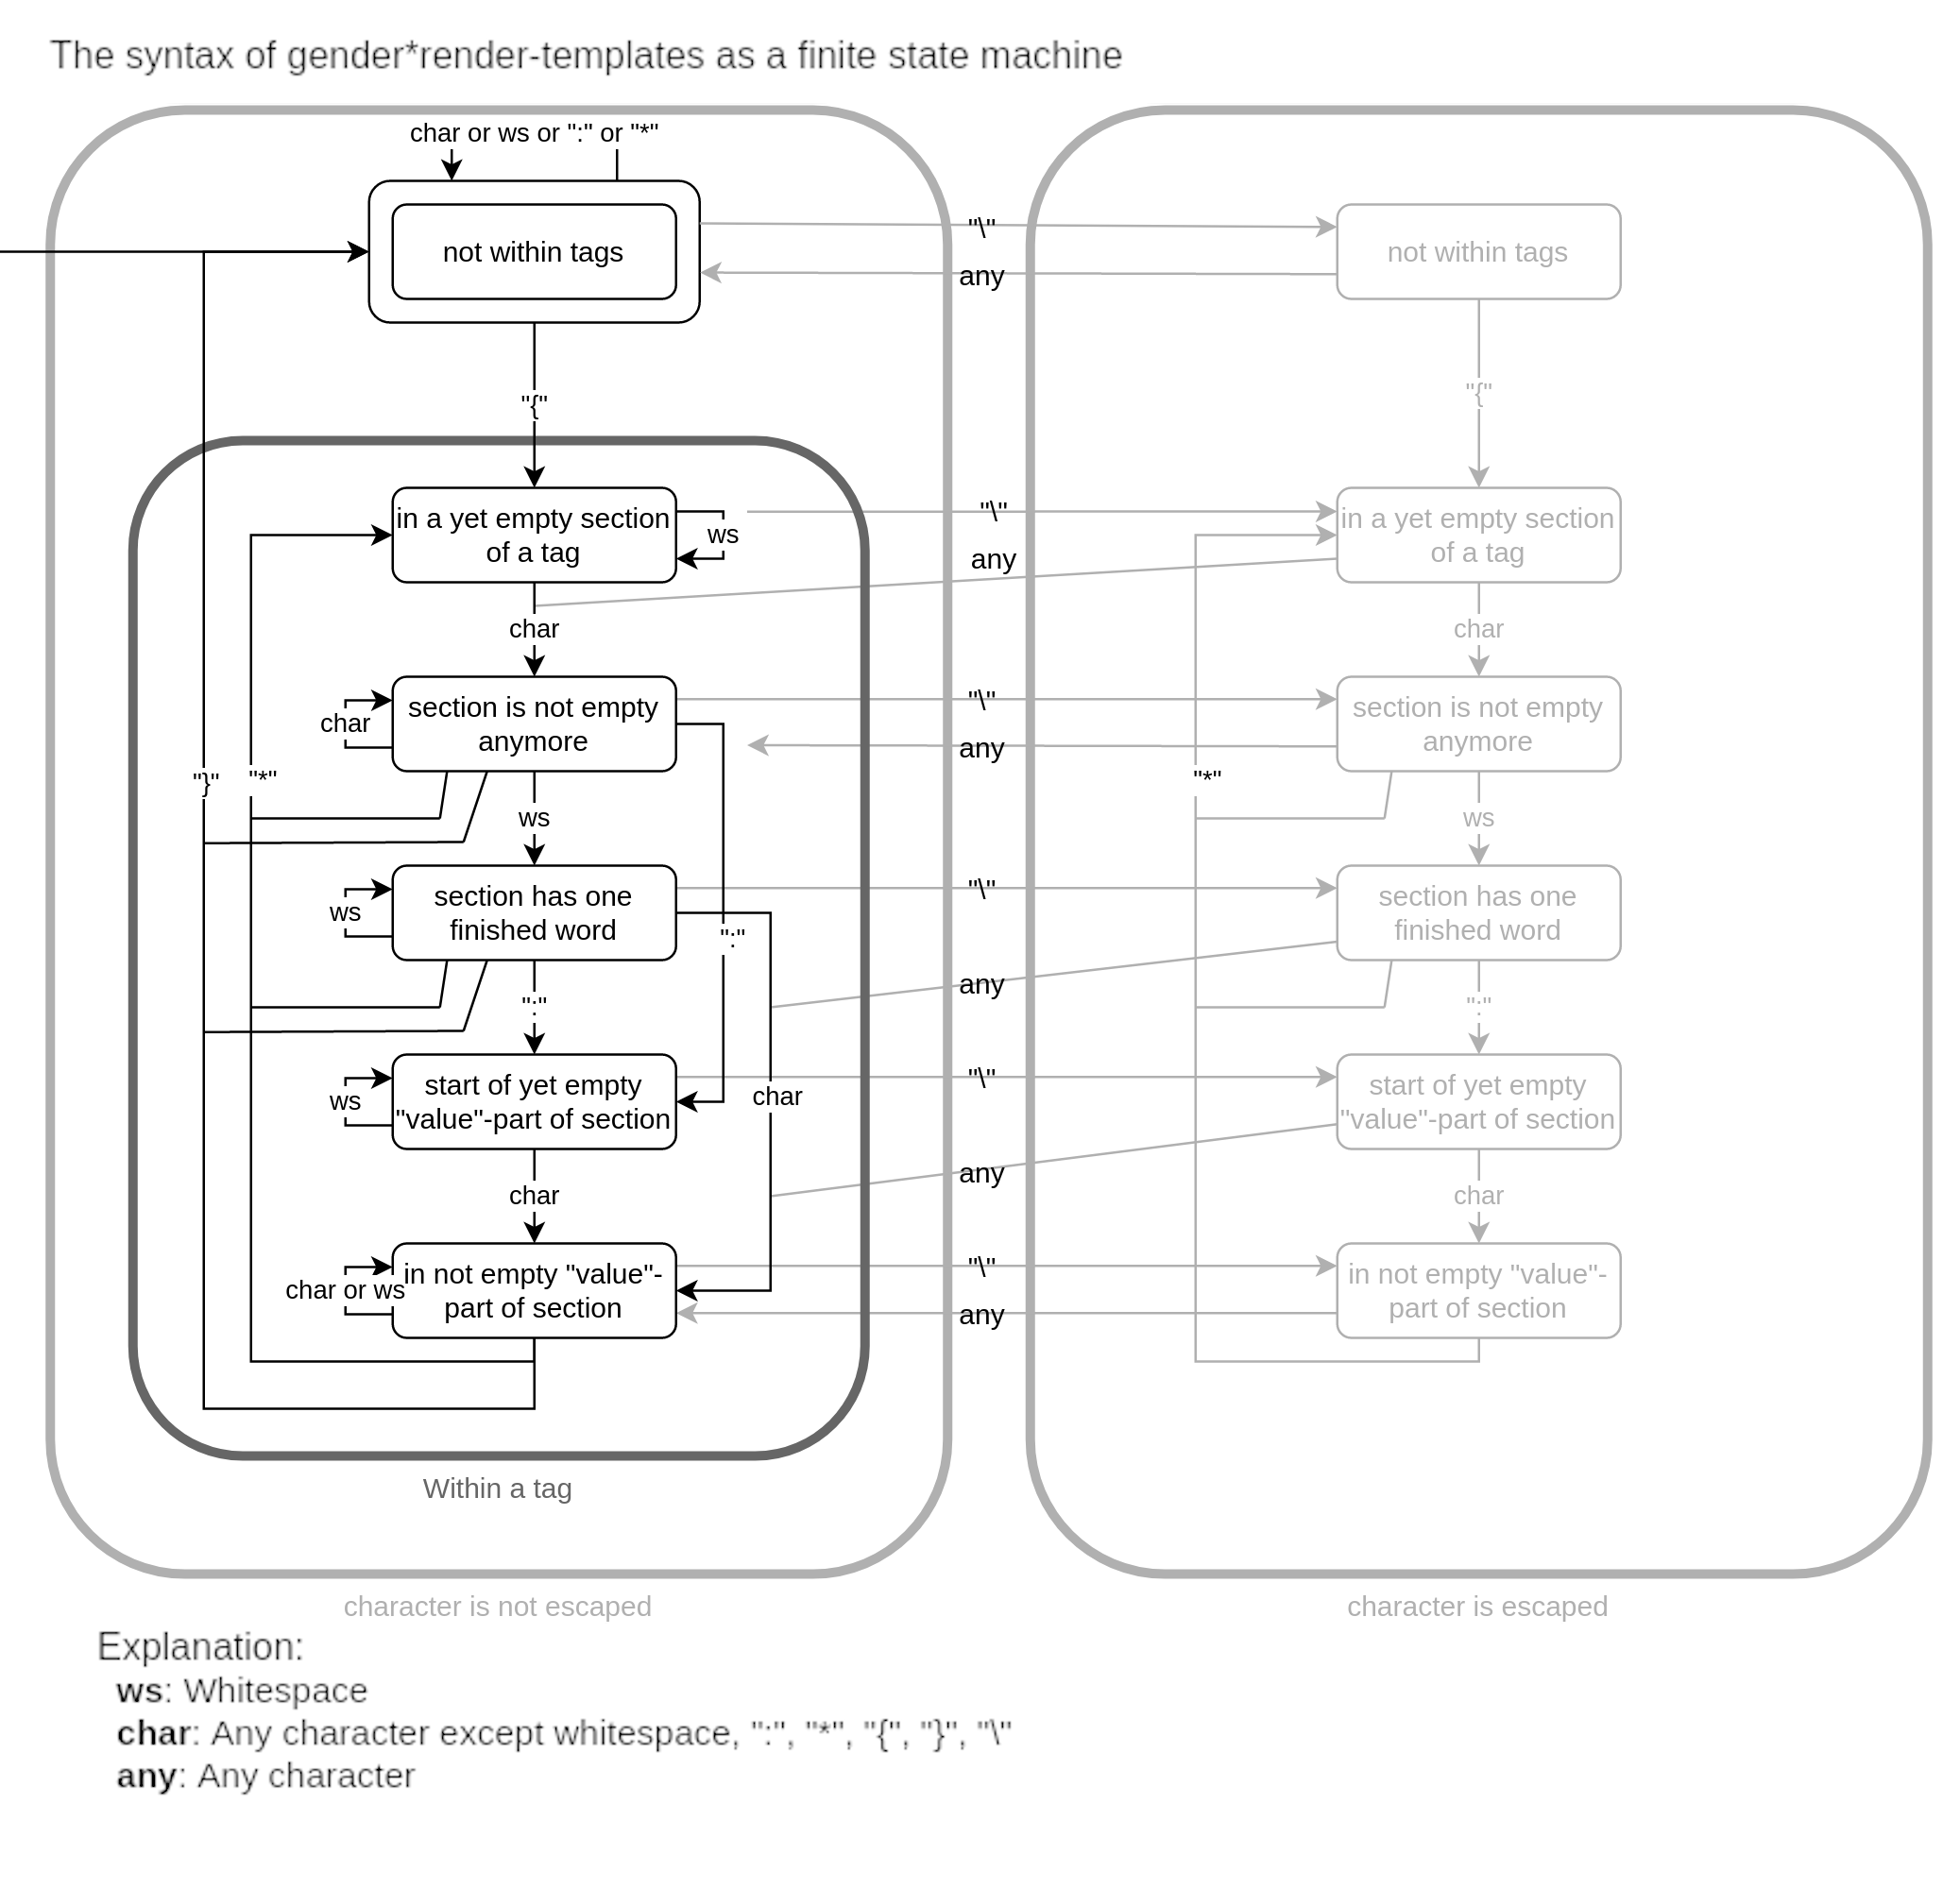
\includegraphics[width=12cm]{images/template-as-finite-state-machine.png}

    \subsection{Pronoun Description Data}

     Pronouns description data, to which we will refer as \{gender*render\}-pronoun-data for the rest of this essay to spare us some words, is the way the user tells the render the pronouns of all people mentioned in a template so the renderer can render it.
     Any piece of text that fits the criteria described below is considered \{gender*render\}-pronoun-data, yet not every such piece of text necessarily works with every template, since it must provide the information required by the template for the rendering to work.
    Files that contain \{gender*render\}-pronoun-data should use the file extension \texttt{.grpd}.\\

    \{gender*render\}-pronoun-data is a type of json data, which makes it easily parsable by any language.\\

    To describe a single individuals pronouns (to which we will refer to as individual pronoun data), a json object is used;
    several of these are then combined to provide pronoun data for all individuals.
    If a piece of individual pronoun data is written into a file, the file extension \texttt{.gripd} should be used.
    Any json object whose properties are strings without whitespace, and whose items are strings, is valid individual pronoun data, though it might not work with every template depending on the information the template requires.\\

    The following table describes the properties a piece of individual pronoun data may use to give you a rough overview of the way individual pronoun data corresponds to the information provided by the \texttt{context}-section of \{gender*render\}-pronoun tags, which will be relevant in the next section (about the way renderers work):


    %\pagebreak[5]
    \begin{flushleft}
        \begin{center}
            \begin{longtable}{|p{7em} | p{9em} | p{14em} |}
                 \hline
                 information provided by properties & property name(s), \linebreak synonymous to each other & short explanation, where necessary\\
                 \hline\hline
                 Subject & they, subject, subj & \\
                 \hline
                 Object & them, object, obj & \\
                 \hline
                 Dependant possessive\linebreak Determiner & their, dposs, dpossessive & \\
                 \hline
                 Independent possessive\linebreak Determiner & theirs, iposs, ipossessive & \\
                 \hline
                 Reflexive & themself, reflexive, reflex & \\
                 \hline
                 \hline
                 Form of Address & Mr, Mrs, Mr\_s, address & \\
                 \hline
                 Surname & Smith, name, surname, family-name & \\
                 \hline
                 Personal name & Avery, personal-name, first-name & \\
                 \hline
                 \hline
                 Gender-specific Noun handling & gender-nouns, gender\_nouns & Describes whether the person wants gender-specific nouns to use the female version where possible (e.g.\ "actress" instead of "actor"), the male version where possible (e.g.\ "fireman" instead of "firefighter"), or the gender-neutral version where possible (e.g.\ "firefighter").
                 Possible values for this property are \texttt{"female"}, \texttt{"male"} and \texttt{"neutral"}. \\
                 \hline
                 \hline
                 Custom property & \emph{property\_name} & Corresponds to "\texttt{<}\emph{property\_name}\texttt{>}" in \{gender*render\}-tags. \\
                 \hline
            \end{longtable}
        \end{center}
    \end{flushleft}

    \{gender*render\}-pronoun-data is simply a json object whose properties are ids (strings without whitespace) corresponding to ids of \{gender*render\}-tags, and whose items are the individual pronoun data corresponding to their respective ids.
    Since the ids used by the \{gender*render\}-pronoun-data need to correspond to those used by the template, not every valid piece of \{gender*render\}-pronoun-data worked with every template.
    As specified later in the spec, renderers accept \{gender*render\}-pronoun-data as well as individual pronoun data in cases where no or only one id is used.

    \subsection{Pronoun Renderer}

    This section describes the way \{gender*render\}-specification conforming pronoun renderers work.
    It is divided into two subsections, one defining a \{gender*render\}-renderer, and one defining (additional) implementation guidelines that should be followed to ensure that all renderers use similar interfaces and users understand the renderer even if they used to work with a different implementation beforehand.
    The \{gender*render\} implementation that comes with this specification (\url{https://github.com/phseiff/gender-render}) also follows all of these guidelines.

    \subsubsection{Pronoun Renderer specification}

    Any program that follows the specifications below is considered a \{gender*render\}-renderer.
    The purpose of such programs is to take \{gender*render\}-templates and \{gender*render\}-pronoun data and render them to texts that are gendered correctly according to the preferences voiced in the pronoun data.
    We will refer to \{gender*render\}-renderers simply as renderers for the rest of this section to aid the reading flow.\\

    A renderer must take at least two inputs, a \{gender*render\}-template and a piece of pronoun data.
    As for the piece of pronoun data a renderer accepts, every renderer must accept \{gender*render\}-pronoun data as well as individual pronoun data, which is then processed into full \{gender*render\}-pronoun data following a number of steps explained below.
    The renderer may also be written in a way that allows to pass it a path to a \texttt{.gr}-file containing a \{gender*render\}-template instead of the template directly, or even in a way which exclusively allows this way of usage, though the later is not recommended and does not comply with the implementation suggestions given by this document.
    Analogously, the renderer may be written in a way that allows to pass it a path to a \texttt{.grpd}-file containing \{gender*render\}-pronoun data or a path to a \texttt{.gripd}-file containing individual pronoun data instead of the content of the \{gender*render\}-pronoun data directly, or even in a way which exclusively allows this way of usage, though the later is not recommended and does not comply with the implementation suggestions given by this document.\\

    Along the rendering process, several errors might occur for several reasons.
    The way errors are classified and communicated to the user is not an implementation detail, but a part of the specification, since classifying errors is especially important due the logical, yet sometimes contra intuitive way \{gender*render\} renders templates.
    This specification thus defines not only what should raise an error, but also suggests different error names for different types of errors.\\

    If the language of the implementation allows defining and raising custom error types, these error types must be defined and risen accordingly.
    If the language does not allow to define custom error types, yet allows to return information even if the execution of a program or function fails, the program or function must return information indicating what type of error occurred in a reasonable way.
    However, if the language of the implementation provides a standardized way to indicate a function failed to run, yet does not provide a way to return additional information about the cause of this failure, the implementation should use the standardized way of failing if an error occurs instead of returning information about the cause of failure.\\

    The following types of errors are defined by this specification, and are used as described below.
    Please note that whilst the names of the errors are always written in camel case throughout this specification, the way they are written should be according to the official style guide of the language they are implemented in, if there is any.
    If the naming conventions of the language comply with the names of the errors defined in this specification, or if the language does not have any naming conventions, the names defined in this specification must be used.

    \begin{flushleft}
        \begin{center}
            \begin{longtable}{|p{13em} | p{19em} |}
                 \hline
                 Error name & commonly used for \\
                 \hline\hline
                 \texttt{SyntaxError} & Used if the input not a valid template and pronoun data aren't valid, independent of the way they relate to each other. \\
                 \hline
                 \texttt{IdResolutionError} & Used if matching individual pronoun data to tags does not wo out.\\
                 \hline
                 \texttt{MissingInformationError} & Used if the individual pronoun data a tag refers to does not contain the information the tag requires.\\
                 \hline
            \end{longtable}
        \end{center}
    \end{flushleft}

    If the language of the implementation already has an error type of the name \texttt{SyntaxError}, and this error can be raised by the implementation manually, the implementation does not need to define a custom equivalent of this error type in their own namespace, and may instead use the pre-defined type.
    This is applicable for some languages like Python, and you can safely ige it if it isn't applicable to your language of choice.
    If the language is object-oriented, including custom errors, the errors defined by this specification may be derived from pre-existing error types, where fitting.
    This may be preferable to using pre-defined error types depending on the way your language implements custom error handling.
    Where possible, additional information regarding the cause of failure and how to fix it should be included, but the way this is done is considered an implementation detail.\\

    The rendering process uses different steps, described as follows.
    Please note that the order in which these steps are executed is not relevant;
    as long as the renderer is guaranteed to produce the same input-output-pairs as any render that accords to this definition does, it is up to the programmer how the renderer works internally.
    Each of these steps vaguely corresponds to one of the error types defined above, and raises almost exclusively said error if it happens to be unfinisheable.\\

    The first step is parsing the input values (template and pronoun data) and checking it for correctness.
    If the received pronoun data is neither valid \{gender*render\}-pronoun data nor individual pronoun data, or if the received template is not a valid \{gender*render\}-template, a \texttt{SyntaxError} is risen.
    Please note that for a \{gender*render\}-template to be valid, not only does the syntax as describes via a formal grammar or a finite state machine be matched, but also does the determination of non-explicitly specified section types need work out, as described in the template-part of this specification.\\

    The second step matches \{gender*render\}-tags to individual pronoun data passed to the rnderer.
    The crux of this is checking whether all ids used by the pronoun data match ids used by the template and vice versa, and making sense of individual pronoun data passed to the renderer.
    This step as well as the next one check not only whether the passed information are valid each on their own, but also whether they are matching.
    The procedures defined during this part of the specification walk a thin, yet clear, line between being too static and therefore forcing the user to provide not required information and reduce the ease of use of \{gender*render\}, and being to lash and therefore making debugging unnecessarily difficult.
    Understanding this part of the specification is crucial for using \{gender*render\}, and the information it gives should therefore be part of communicating the way \{gender*render\} can be used by implementation documentations.\\

    The first part of this step is to deal with the fact that different amounts of \texttt{id} values can be used by different tags, and some tags don't have id values specified, and the given pronoun data might be individual pronoun data and therefore not specify any id values.
    To resolve this issue, the renderer assigns every \{gender*render\}-tag an id value if it doesn't have one already, and converts the given pronoun data to \{gender*render\}-pronoun data if it is individual pronoun data.
    The way this is done is described by the following table, which refers to the amount of id values specified by all \{gender*render\}-tags used in the given template as \#ids:

    \begin{flushleft}
        \begin{center}
            \begin{longtable}{|p{6em} | p{7em} | p{7em} | p{7em} | p{7em} |}
                 \hline
                 & \textbf{\#ids = 0} & \textbf{all tags have the same id assigned} & \textbf{all tags have ids assigned, but not all the same} & \textbf{some tags have ids assigned, some not}\\
                 \hline
                 \textbf{only individual pronoun data is given} & & & &\\
                 \hline
                 \textbf{pronoun data is given for one id (="foo")} & & & &\\
                 \hline
                 \textbf{pronoun data is given for n ($\geq$ 1) ids} & & & &\\
                 \hline
            \end{longtable}
        \end{center}
    \end{flushleft}

\end{document}
